\section{Recasting Inside the Experimental Collaborations}
\label{sec:ch5-recastingInsideExp}

Reinterpretations performed within the experiments themselves present unique advantages and disadvantages. They allow for thorough and consistent treatment of detector effects and geometry, object reconstruction, and systematic uncertainties in a way which is impossible through external recasting. Groups can share resources and easily communicate all necessary details. On the other hand, they are of course limited to the model(s) chosen for reinterpretation. In the ideal situation, reinterpretation(s) which provide meaningful results can be performed with minimal overhead to a given analysis.

As the LHC enters an era of deccelerating luminosity growth and following  trends towards more sophistication in analysis techniques, the LHC analyses become harder to re-implement with sufficient accuracy outside of the experiments compared to cut-based analyses. Analyses increasingly utilize machine-learning algorithms that transform a large number of event-level and particle-level observables into higher-level discriminants, which are not easily characterized by low-dimensional efficiency tables and may require inputs that third-party detector simulations are not able to reproduce. In particular non-prompt searches may depend on non-traditional reconstruction objects and details of the detector simulation and geometry in ways that require a more detailed simulation than is achievable by, \emph{e.g.}, third-party simulators. Hence, experiments are investigating approaches that enable internal re-interpretation using the full set of available information.

Full-fidelity reinterpretations are  especially relevant for long-lived particles, since the signal simulation may depend more heavily on details not well captured by third-party simulation tools. For example, for sufficiently high lifetime, the decays must be handled by a full detector simulation such as GEANT (or some complex interaction between GEANT and MC packages such as Pythia). Such decays are not well-covered by tools like Delphes as the response of such in-detector decays may require access to a more detailed geometry description.

\subsection{The RECAST Framework}

The RECAST Framework~\cite{Cranmer:2010hk} is a developing platform for experiments as well as  researchers external to the collaborations who wish to reinterpret LHC analyses. RECAST enables cloud-based analysis execution and common presentation of reinterpretation results. The framework consists of two components:

\paragraph{The RECAST Front-End} This is a web-based service in which reinterpretation of analyses can be suggested by interested authors that provide necessary inputs such as UFO model files \cite{Degrande:2011ua}, process and parameter card templates, or suggested scan grids. Responses to such requests, possibly by more than one analysis implementation, can then be uploaded. Such a web service, interfaced with services such as HepData, may then serve as a resource for the LHC community to organize and share reinterpretation results obtained by the various analysis implementations.

\paragraph{The RECAST Back-end} An important objective of the framework is to enable a full-fidelity reinterpretation of an LHC analysis using the original analysis code developed within the experiment that can be approved by the collaboration and be placed on an equal footing with the original publication. In contrast to third-party recasting tools, in which multiple analyses are implemented using a single, common framework that is  executed on a single computing element, such an exact analysis re-execution often necessitates a distributed data analysis using a number of different frameworks in use within the experiments. Therefore, RECAST has developed a flexible graph-based, analysis description and execution backend~\cite{Heinrich:2297545} that enables a faithful re-execution of nearly arbitrary analysis code on cloud platforms such as those offered by CERN\footnote{Thanks to this flexibility, the popular third-party recasting tools can  be easily integrated into this back-end as well, with current integrations being available for CheckMate and Rivet.}. The back-end provides experiments with an access-controlled interface to view reinterpretation requests, retrieve the necessary analysis description from repositories such as the CERN Analysis Preservation Portal (CAP)~\cite{CAP},  execute the analysis on datasets for the new model and -- if approved -- upload the results to the public front-end. Figure~\ref{fig:recast-cc} shows a screenshot of the current prototype user interface, giving collaboration members an overview over requested points as well as controls to steer processing and submission.

\begin{figure}[t]
\begin{center}
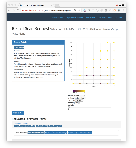
\includegraphics[width=0.5\textwidth,angle=0]{ch5-figures/requestview.pdf}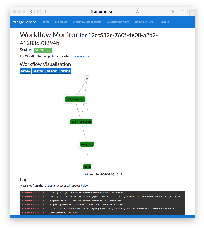
\includegraphics[width=0.5\textwidth,angle=0]{ch5-figures/monitor.pdf}

\end{center}
\caption{
Left: web-based interface for RECAST backend for experiment that presents the requested parameter points and color-coded results,
Right: an experiment-internal reinterpretation executing on the distributed infrastructure built by CAP and RECAST.}
\label{fig:recast-cc}
\end{figure}

These services are being developed in close collaboration with the CERN Analysis Preservation project, which is a common project supported by the four major LHC experiments. While this integration work is on-going, the computing backend for RECAST has been successfully used for a number of Run 1 and Run 2 reinterpretations published by the ATLAS Experiment.


\subsection{Analysis Preservation as a Driver for Re-Interpretation}

Within the LHC experiments, the ability to re-interpret analyses is, perhaps unintuitively, mostly limited by the internal availability of the analysis routines to the wider collaboration as opposed to, \emph{e.g.}, availability of computing resource constraints. The large number of measurements and searches, the heterogeneity and complexity of the analysis software, as well the size of the collaboration all lead to a situation in which  only a small number of analyzers of the original analysis team are often-times able to execute any given analysis. Furthermore, due to the collaborative development model, analyzers  are typically responsible for only a subset of the analysis, which results in knowledge fragmentation. Therefore, both ATLAS and CMS are now designing an interface to store analysis-relevant information (the CERN Analysis Preservation Portal, CAP~\cite{CAP}) to mitigate this problem. In the context of RECAST, the software and analysis-workflow preservation aspects of this effort are most relevant. The former is mainly implemented through archiving of source-code repositories and the archival Linux Containers, which now enjoy wide-spread industry support, while internal structure of the analysis workflow is archived in CAP in the form of declarative workflow specifications such as yadage~\cite{Cranmer:2017frf}, which has been developed for RECAST, and the Common Workflow Language (CWL)~\cite{CWL}. It is planned that CAP and RECAST will utilize a common computing back0end in order to re-execute the analyses that have been preserved in the portal. As the preservation is enabled by recent technological advances and the process of archival is increasingly streamlined, it is expected that a higher number of  experiment-internal analysis codes will be available for RECAST.



\subsection{RECAST Examples}

\paragraph{ATLAS-Internal Analysis Examples and Results :}

A number of re-interpretation publications have been supported by the backend underpinning RECAST. After Run 1, ATLAS has conducted a thorough re-interpretation of the SUSY landscape in the context of the phenomenological pMSSM~\cite{Aad:2015baa}, a study involving 20 SUSY analyses and 50,000 fully simulated pMSSM parameter points. While at that time, most analyses had to be re-interpreted manually, the 2L electroweak analysis~\cite{Aad:2014vma} included in that paper served as a prototype analysis and provided results using the highly automated RECAST back-ends.

The analysis was than later re-used with minimal additional effort in two additional publications that focused on more domain-specific SUSY realizations:~a five-dimensional dark-matter reinterpretation of electroweak seaches~\cite{Aaboud:2016wna}, as well as a reinterpretations in the context of general gauge-mediated models~\cite{ATLAS-CONF-2016-033}.

\begin{figure}[t]
\begin{center}
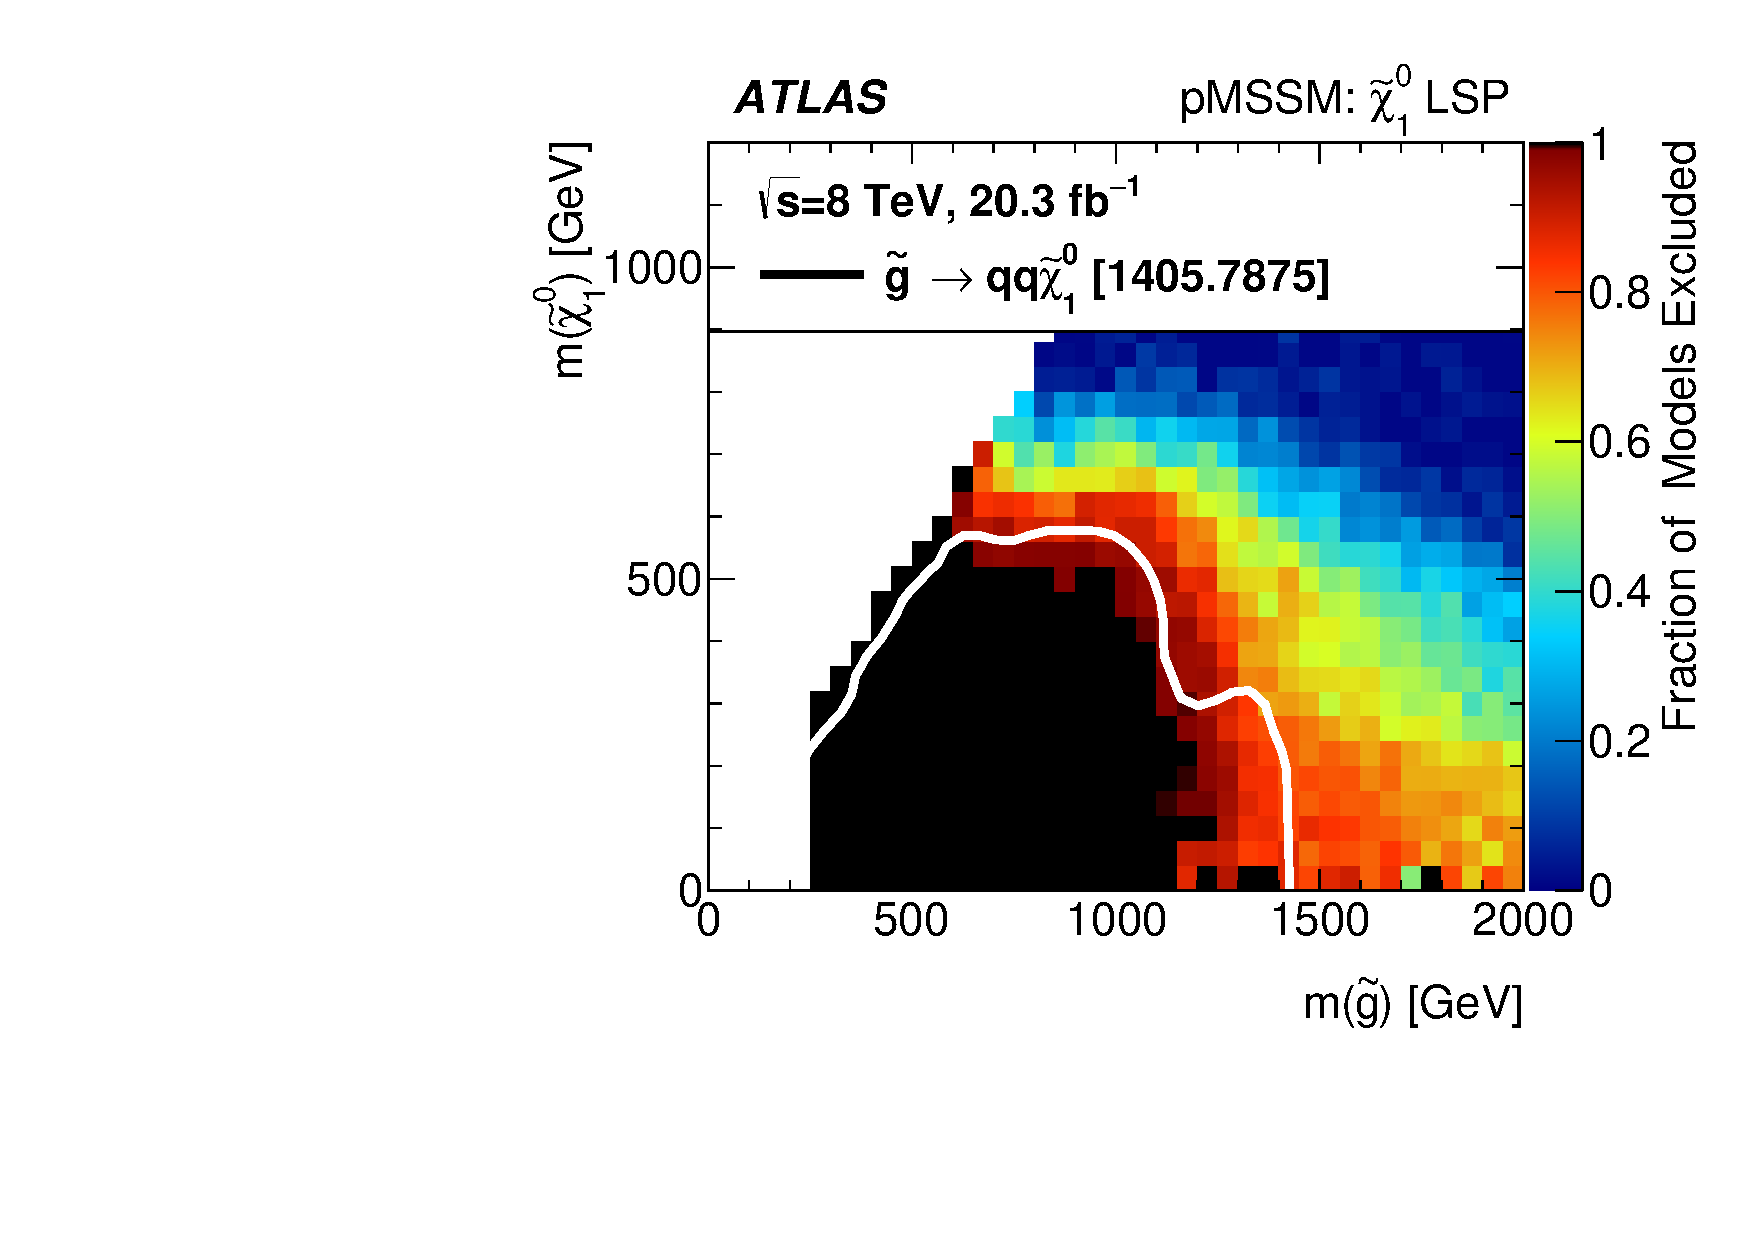
\includegraphics[width=0.48\textwidth,angle=0]{ch5-figures/pMSSM.pdf}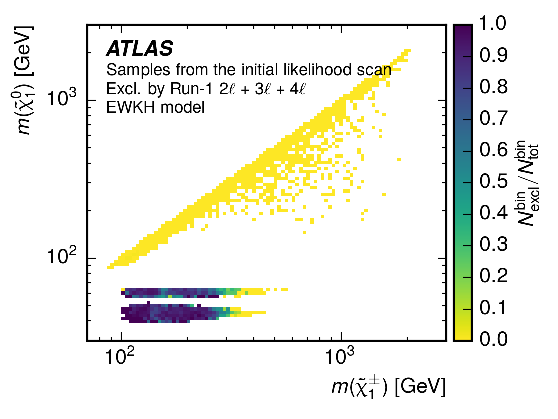
\includegraphics[width=0.52\textwidth,angle=0]{ch5-figures/DM.pdf}

\end{center}
\caption{
Left: pMSSM exclusion in the gluino-neutralino mass-plane. Results partially provided by RECAST.
Right: follow-up dark-matter re-interpretation. Exclusions presented in chargino-neutralino mass-plane.
}
\label{fig:recast-cc}
\end{figure}



Recently ATLAS has reinterpreted 10 analyses~\cite{ATLAS-CONF-2018-003} in terms of models of supersymmetry with non-vanishing baryon-number violating coupling strength $\lambda''$ partly through the use of the new analysis preservation infrastructure. In such models the lighest neutralino it unstable with a decay length of

\begin{equation}
  L(cm) = \frac{0.9\beta\gamma}{{\lambda''}^2} \left(\frac{m(\bar{q})}{100\mathrm{GeV}}\right)^4\left(\frac{1\mathrm{GeV}}{m(\tilde{\chi}_1^0)}\right)^5.
\end{equation}

This reinterpretation required a joint re-execution of a mix of analyses originally designed for R-parity-conserving and R-parity-violating models and special systematics have been added into the statistical analyses to account for the detector response and flavor-tagging rate of displaced-ets. Results were presented in a two-dimensional parameter space of gluino mass and neutralino lifetime (or analogously the $\lambda''$ coupling) as shown in Figure~\ref{fig:rpvrpc}. Such reinterpretations are difficult to perform outside of the experiments, as the publicly available information lack details of the detector and analayses.

\begin{figure}[h]
\begin{center}

\includegraphics[width=0.85\textwidth,angle=0]{ch5-figures/fig_04.pdf}
\end{center}
\caption{Exclusion limits as a function of $\lambda''_{323}$ and $m({\tilde{g}})$. Expected limits are shown with dashed lines, and observed as solid. Taken from Ref.~\cite{ATLAS-CONF-2018-003}.}
\label{fig:rpvrpc}
\end{figure}



\paragraph{Third-Party Tool Integration }

Both the CheckMate~\cite{Drees:2013wra,Dercks:2016npn} and the Rivet~\cite{Buckley:2010ar} analysis catalogues have been implemented in the analysis-execution framework. Both are configured to analyze events that are provided in the HepMC format
\cite{Dobbs:2001ck}. Due to the modular approach of the analysis back-end, a number of MC generation workflows, such as Herwig~\cite{Marchesini:1991ch}, SHERPA~\cite{Gleisberg:2008ta} or MadGraph~\cite{Alwall:2011uj}, can be used depending on their ability to correctly model the desired signal.

For analyses where multiple implementation exists, \emph{e.g.,} from multiple third-party tools such as Rivet BSM, CheckMate or MadAnalysis~\cite{Conte:2014zja,Dumont:2014tja} as well as from multiple experiment-internal configurations (fast Simulation, full simulation), RECAST will allow the community to compare and contrast reinterpretation results.

\subsection{Outlook}

Thanks to industry-backed technological advances, a realistic technical solution to the Analysis Preservation problem for the LHC experiments and the original RECAST proposal has come into view. The initial use of such infrastructure for the reinterpretation for prompt SUSY searches is generalized easily for long-lived particle searches as the tools used for  signal simulation, analysis preservation, and execution do not make simplifying assumptions on the nature of the BSM signal or analysis structure.  As such, RECAST may cover reinterpretation use-cases, where either third-party reinterpretations are impossible due to missing public information or limitations of third-party tools or accurate, experiment-approved results are desired.
